\subsection{Class Diagram}
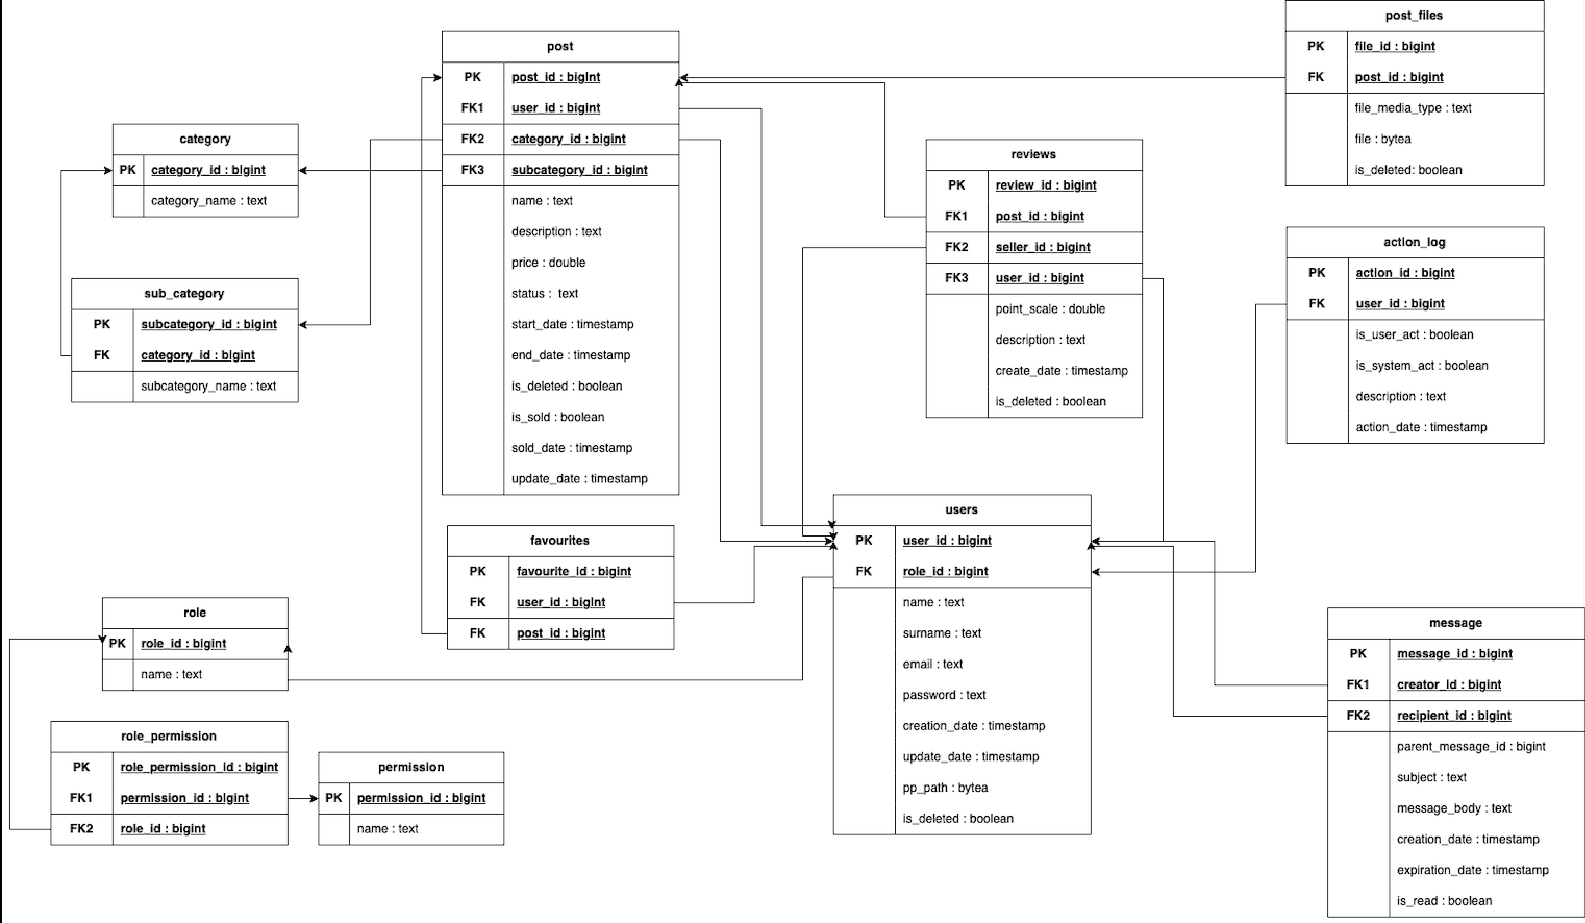
\includegraphics[scale = 0.65]{classDiagram.pdf}
\begin{center}
\caption{Class Diagram}
\end{center} 
\hspace{5mm}As a software engineering definition, “class diagram” in UML architecture structural design that describes the structure of a system by showing the overall systems classes, their attributes, operations (or methods), and the relationships among objects. For our project we made class diagram for our Resources with their attributes and their types. \newline



%Describe here the class diagram of your project

%if needed write here other details about your Data Logic Layer that cannot be expressed directly through the ER schema
Activity diagrams are one of the most significant diagram in UML architecture for the representation of dynamic aspects of the overall system in parts. Dynamic operations which are also can be denoted as the activities can be shown as flowchart representations before the real development of the system. That is why in each activity diagram there exist a start and end point that encapsulates the overall activity flow in each represented part.
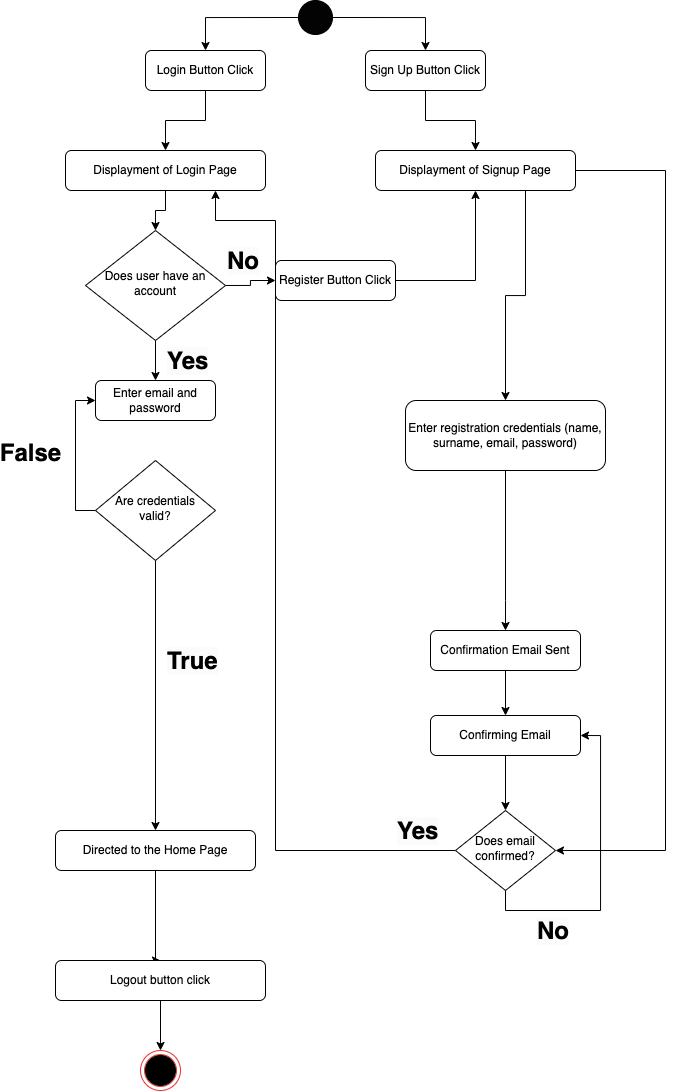
\includegraphics[scale=0.65]{loginFlow.png} \newline



In the above, activity diagram represents the flow of the login and registration operations within the system. As shown in the diagram, they work in a coherent way and interacts with each other. \newline

Further Development Plans: Google Authentication for the login operation and Google Registration for the registration operation will be implemented. And email service will be supplied with external email services.\newline

\rotatebox[origin=c]{90}{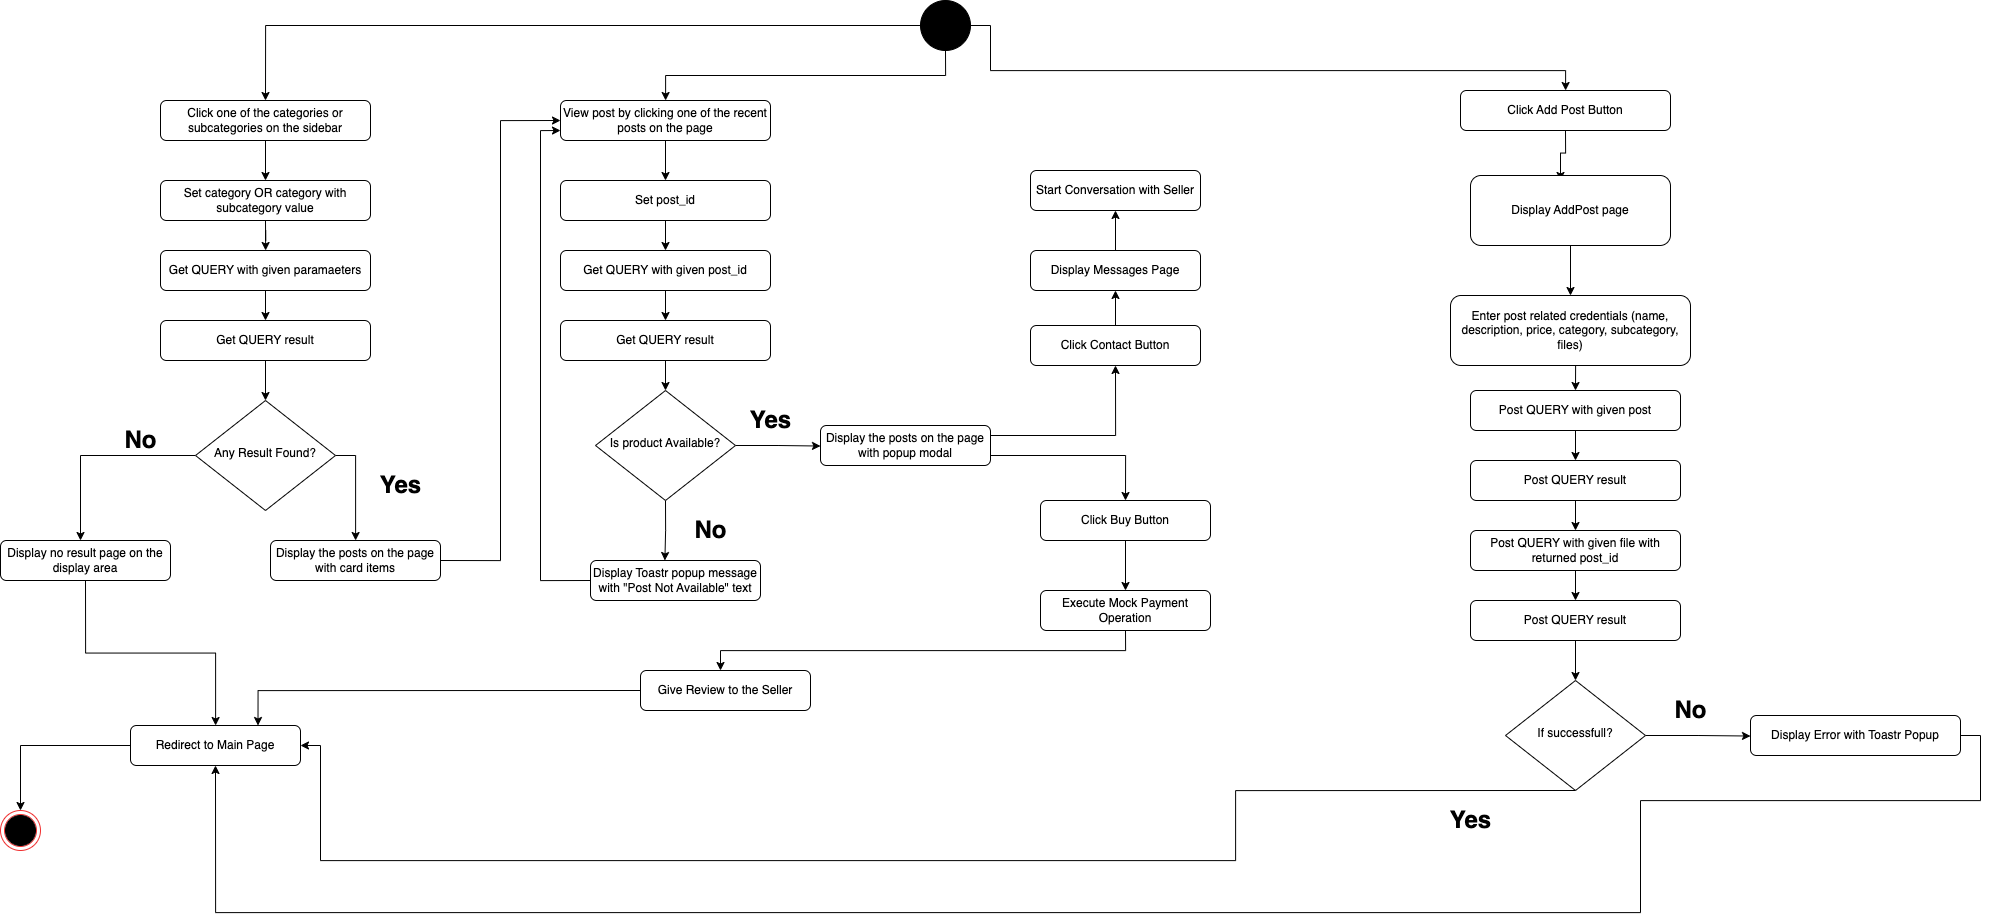
\includegraphics[scale=0.38]{postmainFlow.png}}\\

Above diagram demonstrates the post related flows that can be accessed from the main page of the system. Post operations can be overviewed as by viewing and adding activities. Additional operations on the posts such as buying and contacting with the seller will be directed to their services and related pages. If the view operation observed from the perspective of authorized user, user is authorized for editing his/her post. \newline

If we observe the flows in parts user is authorized for post addition, viewing other users posts and viewing authenticated users posts. 
By viewing other post user can either buy or contact with the seller for further informations. When the post related operation finished user will be redirected to the main page and activity will be set as finished. \newline

Further Development Plans: Buy operation will be handled by an external payment service. Java payment libraries will be overview and chosen accordingly.\newline

\rotatebox[origin=c]{90}{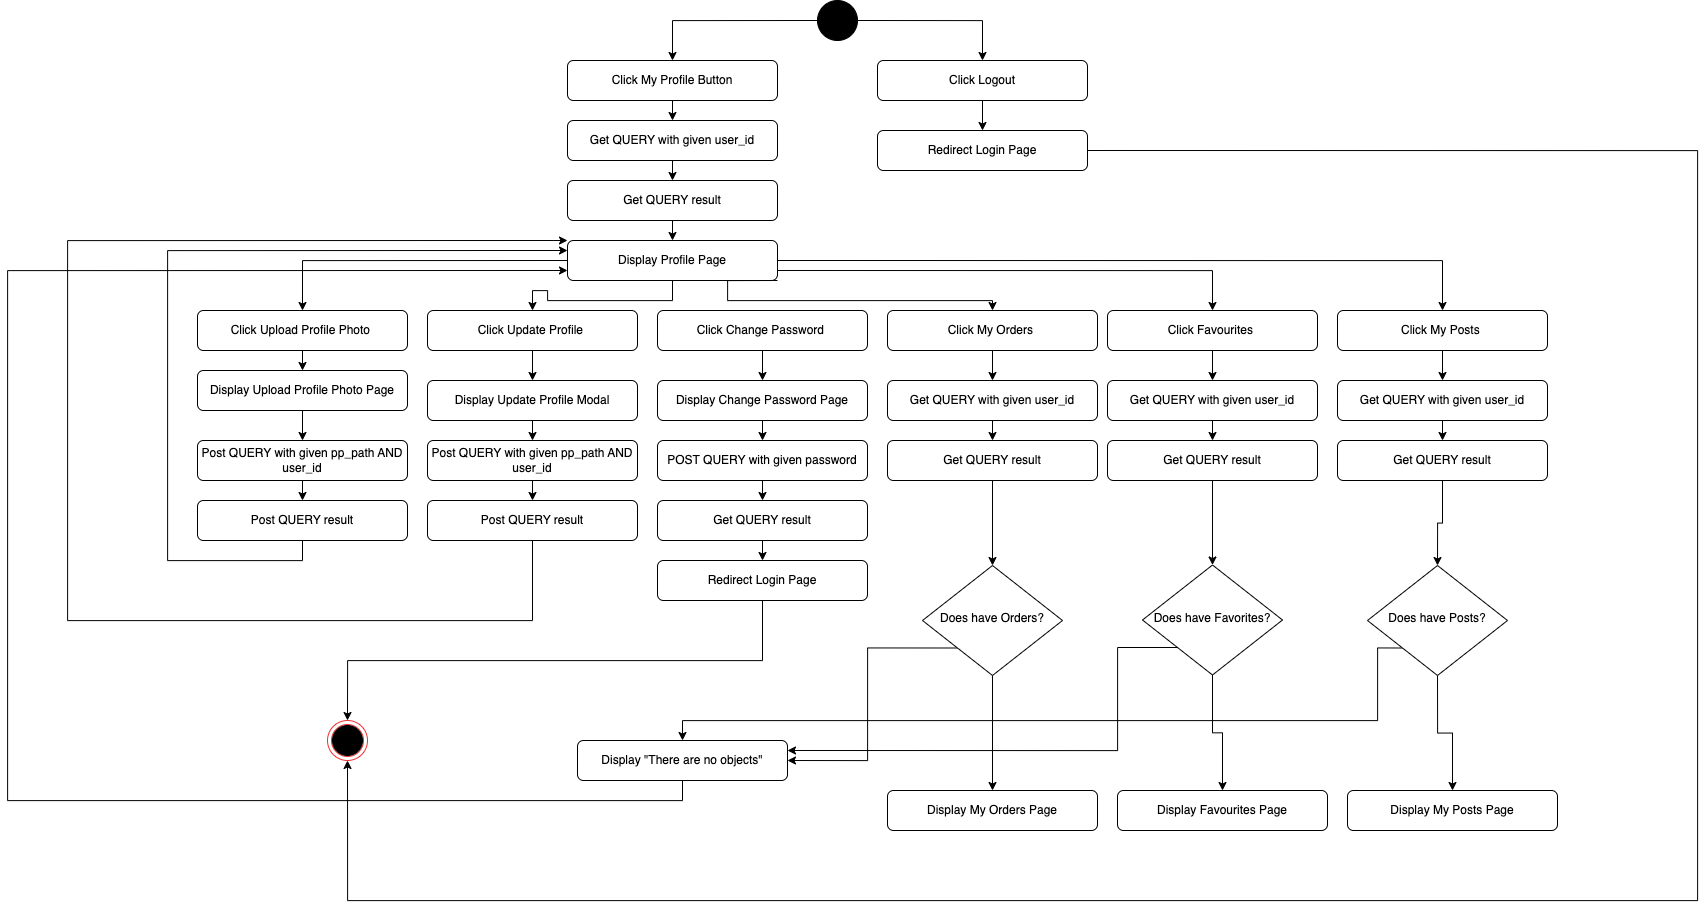
\includegraphics[scale =0.45 ]{profileFlow.png}}\newline

Above diagram demonstrates the profile related flows that can be accessed from the profile page of the user. All user related profile operations can be listed as updating information, changing password, updating profile photo, viewing the aftermath of the operations of purchasing, contacting and adding posts. Every operation in the activity flow triggers the specific queries that will redirect the changes to the profile page. \newline

As an important operation, changing password triggers the logout operation automatically that also navigates user to the login page again. \newline


